\pgfkeys{/pgf/declare function={rescale(\x) = (\x*2-1)^3*0.5+0.5;}}

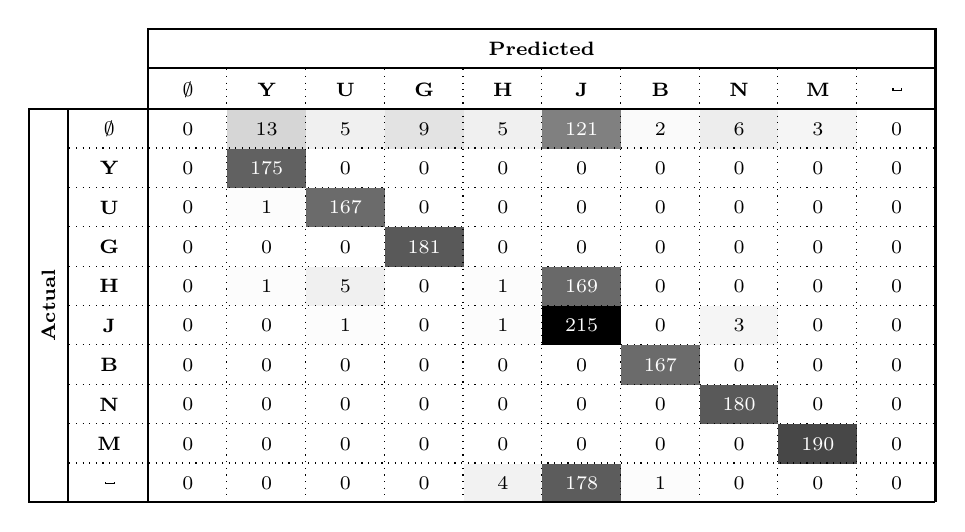
\begin{tikzpicture}[
    square/.style={
        inner sep=0pt,
        rectangle,
        minimum width=1cm,
        minimum height=0.5cm,
        anchor=north west,
    },
    every node/.style={
        font=\scriptsize,
    },
]
    % \node[inner sep=2pt,circle,fill=green] at (0, 0) {};
    \node[inner sep=0pt,rectangle,anchor=south east,rotate=90,minimum width=5cm,minimum height=0.5cm,draw,xshift=0.5\pgflinewidth,thick]
        at (0, -0.5) {\bfseries{}Actual};
    \node[inner sep=0pt,rectangle,anchor=south west,minimum width=10cm,minimum height=0.5cm,draw,xshift=-0.5\pgflinewidth,thick]
        at (1, 0) {\bfseries{}Predicted};

    \foreach \row [count=\y] in {{0,13,5,9,5,121,2,6,3,0},{0,175,0,0,0,0,0,0,0,0},{0,1,167,0,0,0,0,0,0,0},{0,0,0,181,0,0,0,0,0,0},{0,1,5,0,1,169,0,0,0,0},{0,0,1,0,1,215,0,3,0,0},{0,0,0,0,0,0,167,0,0,0},{0,0,0,0,0,0,0,180,0,0},{0,0,0,0,0,0,0,0,190,0},{0,0,0,0,4,178,1,0,0,0}} {
        \foreach \v [count=\x] in \row {
            \pgfmathsetmacro{\tmp}{\v/215.0}
            \pgfmathtruncatemacro{\back}{rescale(\tmp)*100}
            \pgfmathtruncatemacro{\fore}{(\tmp>0.5)*100}
            \node[square,fill=black!\back!white,text=white!\fore!black] at (\x,-\y*0.5) {$\v$};
        }
    }

    \foreach \key [count=\i] in {$\emptyset$,Y,U,G,H,J,B,N,M,\textvisiblespace} {
        \node[square] at (0, -(\i*0.5) {\bfseries\key};
        \node[square] at (\i, 0) {\bfseries\key};
    }

    \foreach \i in {2,...,10} {
        \draw[draw,dotted] (\i, 0) -- (\i, -5.5);
        \draw[draw,dotted] (0, -\i*0.5) -- (11, -\i*0.5);
    }

    \foreach \i in {1,11} {
        \draw[draw,thick] (\i, 0) -- (\i, -5.5);
        \draw[draw,thick] (0, -\i*0.5) -- (11, -\i*0.5);
    }
\end{tikzpicture}
